\graphicspath{{content/3_results/figures}}
\section{Range Sensor}\label{sec:range_sensor_results}

\subsection{Simulation}

\begin{figure}[!htb]
    \centering
    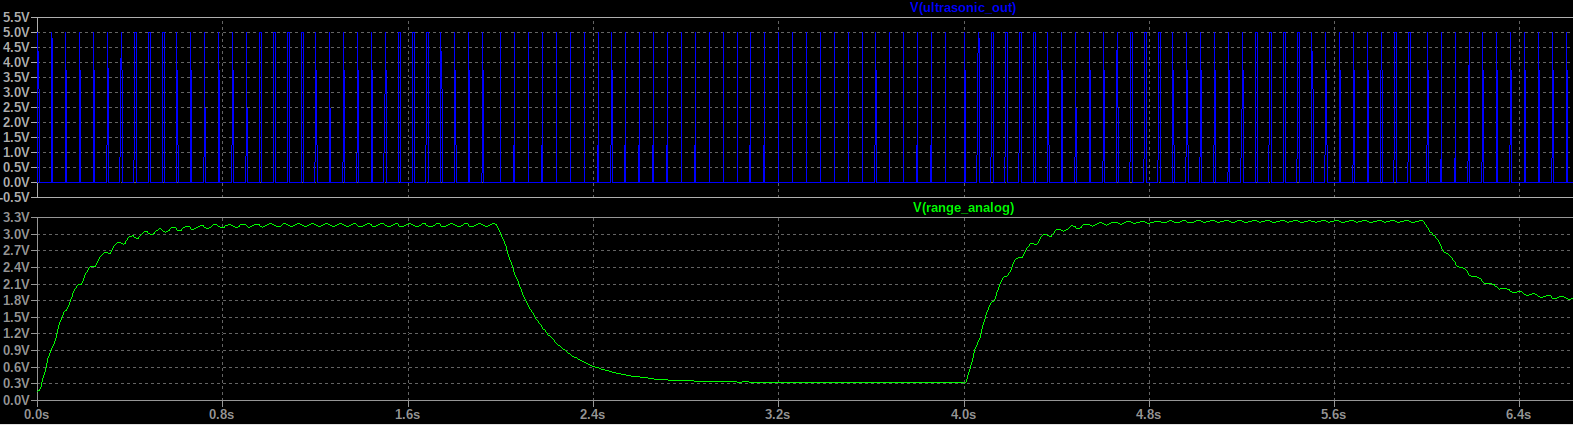
\includegraphics[width=0.8\textwidth]{rangeSensor_sim_fullRange}
    \caption{Full-Range PWM using Modified Workbench}
    \label{fig:rangeSensor_sim_fullRange}
\end{figure}

\begin{figure}[!h]
    \centering
    \begin{minipage}{0.45\textwidth}
        \centering
        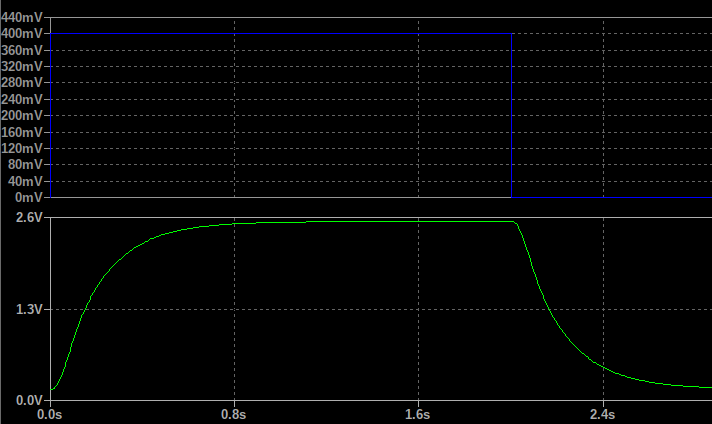
\includegraphics[width=0.8\textwidth]{rangeSensor_sim_stepResponse}
        \caption{400 mV Step Response Input vs Output}
        \label{fig:rangeSensor_sim_stepResponse}
    \end{minipage}
    \begin{minipage}{0.45\textwidth}
        \centering
        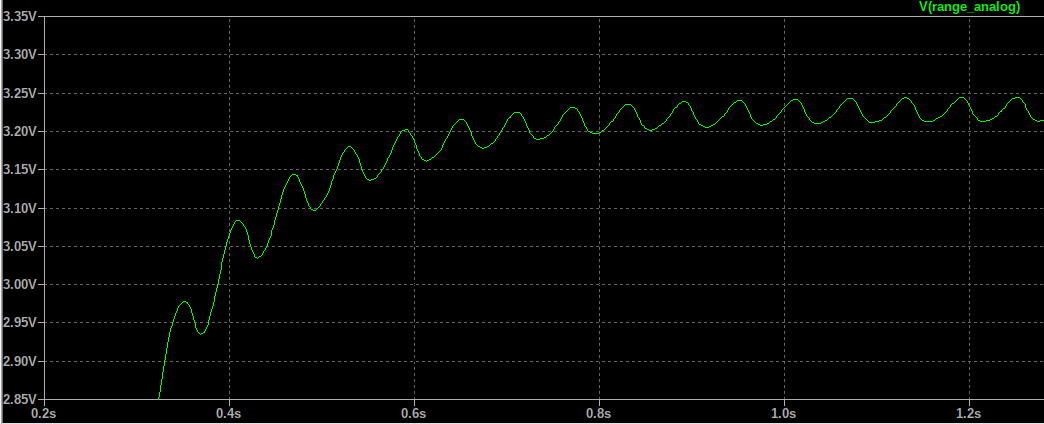
\includegraphics[width=1.0\textwidth]{rangeSensor_sim_noiseLevel}
        \caption{Noise Level}
        \label{fig:rangeSensor_sim_noiseLevel}
    \end{minipage}
\end{figure}

\begin{figure}[!htb]
    \centering
    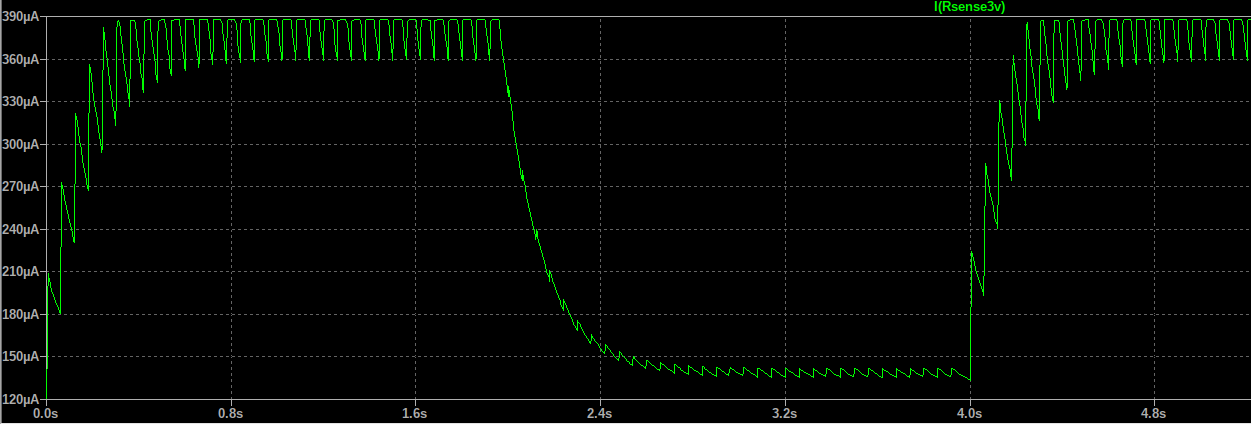
\includegraphics[width=0.5\textwidth]{rangeSensor_sim_currentDraw}
    \caption{Current Draw}
    \label{fig:rangeSensor_sim_currentDraw}
\end{figure}

As seen in the above figures, all specifications were complied with:
\begin{itemize}
    \item Figure \ref{fig:rangeSensor_sim_fullRange} demonstrates the default simulation to test the distance limits with $\tau$ = 0.05\% to 9.5\%,
          followed by the original workbench settings. As visible, the output is $\geq$ 3.0 V for far distances, and $\leq$ 300 mV for close distances.
    \item Figure \ref{fig:rangeSensor_sim_stepResponse} shows the response time of around 800 ms, much less than required 1.5 s.
    \item Figure \ref{fig:rangeSensor_sim_noiseLevel} demonstrates the low noise ripple of around 50 mV, less than the required 70 mV.
    \item Figure \ref{fig:rangeSensor_sim_currentDraw} indicates a maximum current draw of $\SI{390}{\micro\ampere}$, less than the maximum $\SI{750}{\micro\ampere}$.

\end{itemize}

\subsection{Measured}

\begin{figure}[!htb]
    \centering
    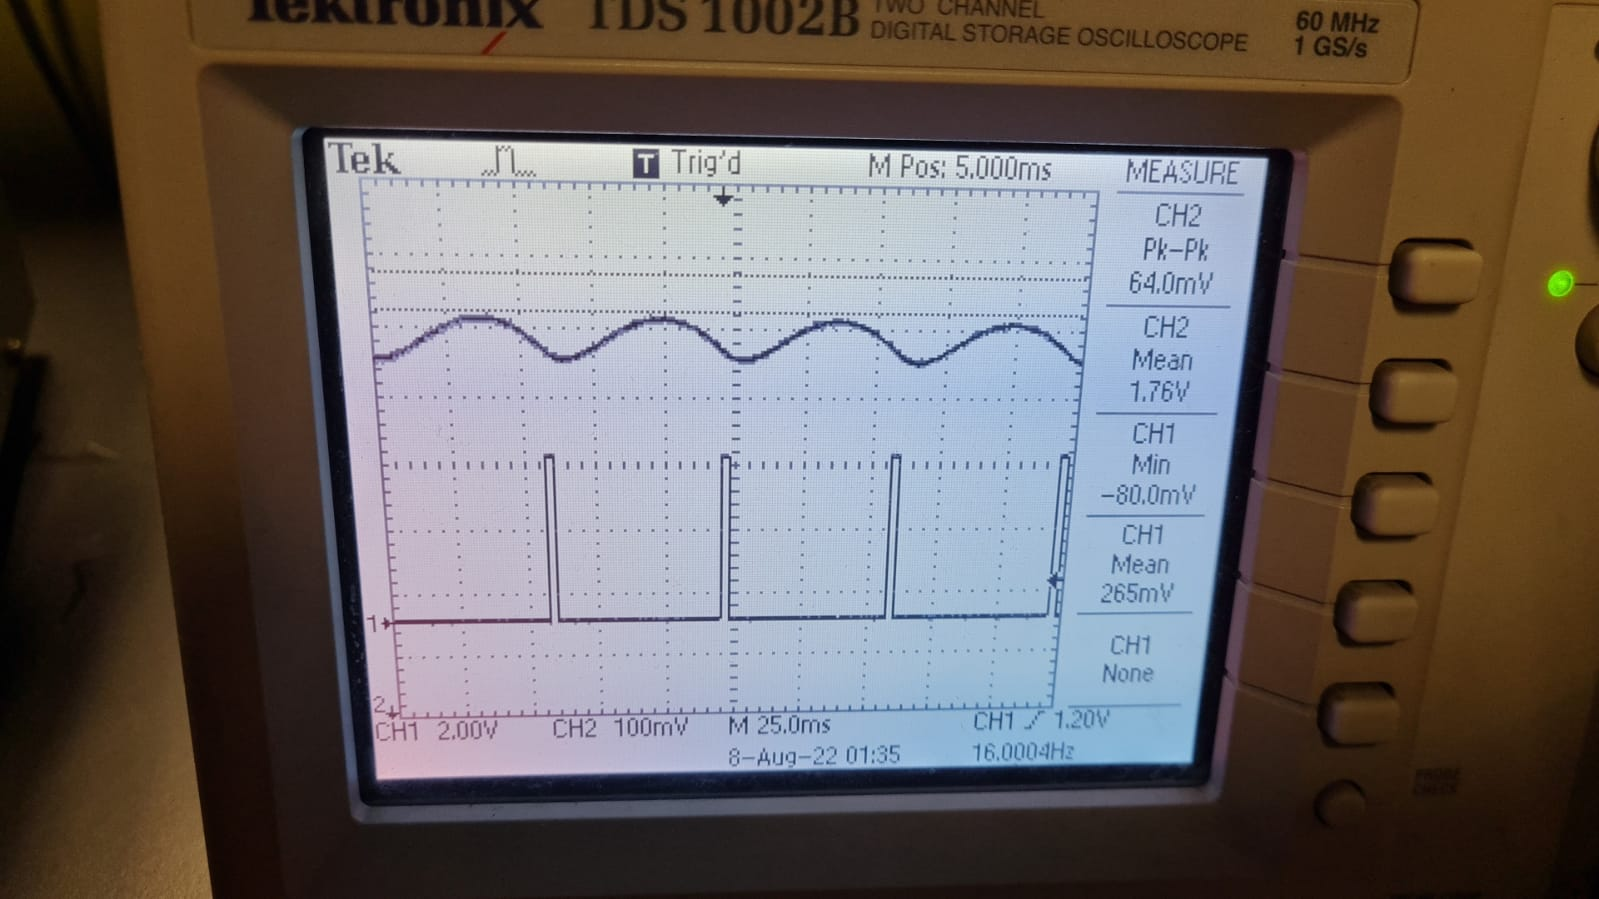
\includegraphics[width=0.6\textwidth]{rangeSensor_impl_noiseLevel}
    \caption{Noise Level}
    \label{fig:rangeSensor_impl_noiseLevel}
\end{figure}

\begin{figure}[!htb]
    \centering
    \begin{minipage}{0.45\textwidth}
        \centering
        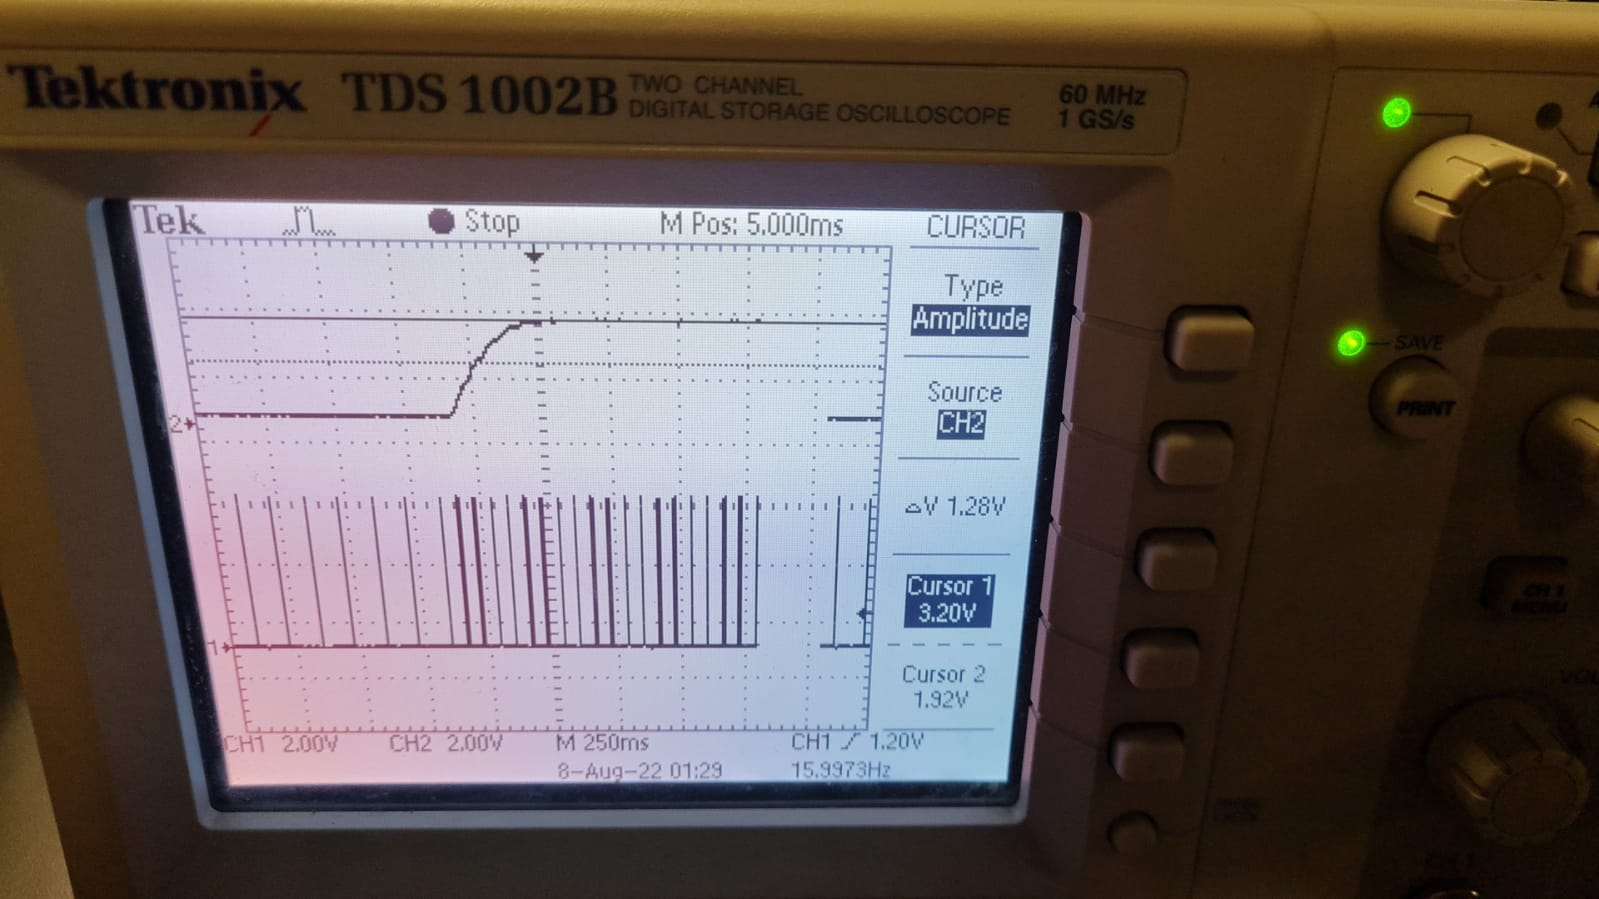
\includegraphics[width=0.95\textwidth]{rangeSensor_impl_stepResponse}
        \caption{Step Response}
        \label{fig:rangeSensor_impl_stepResponse}
    \end{minipage}
    \begin{minipage}{0.45\textwidth}
        \centering
        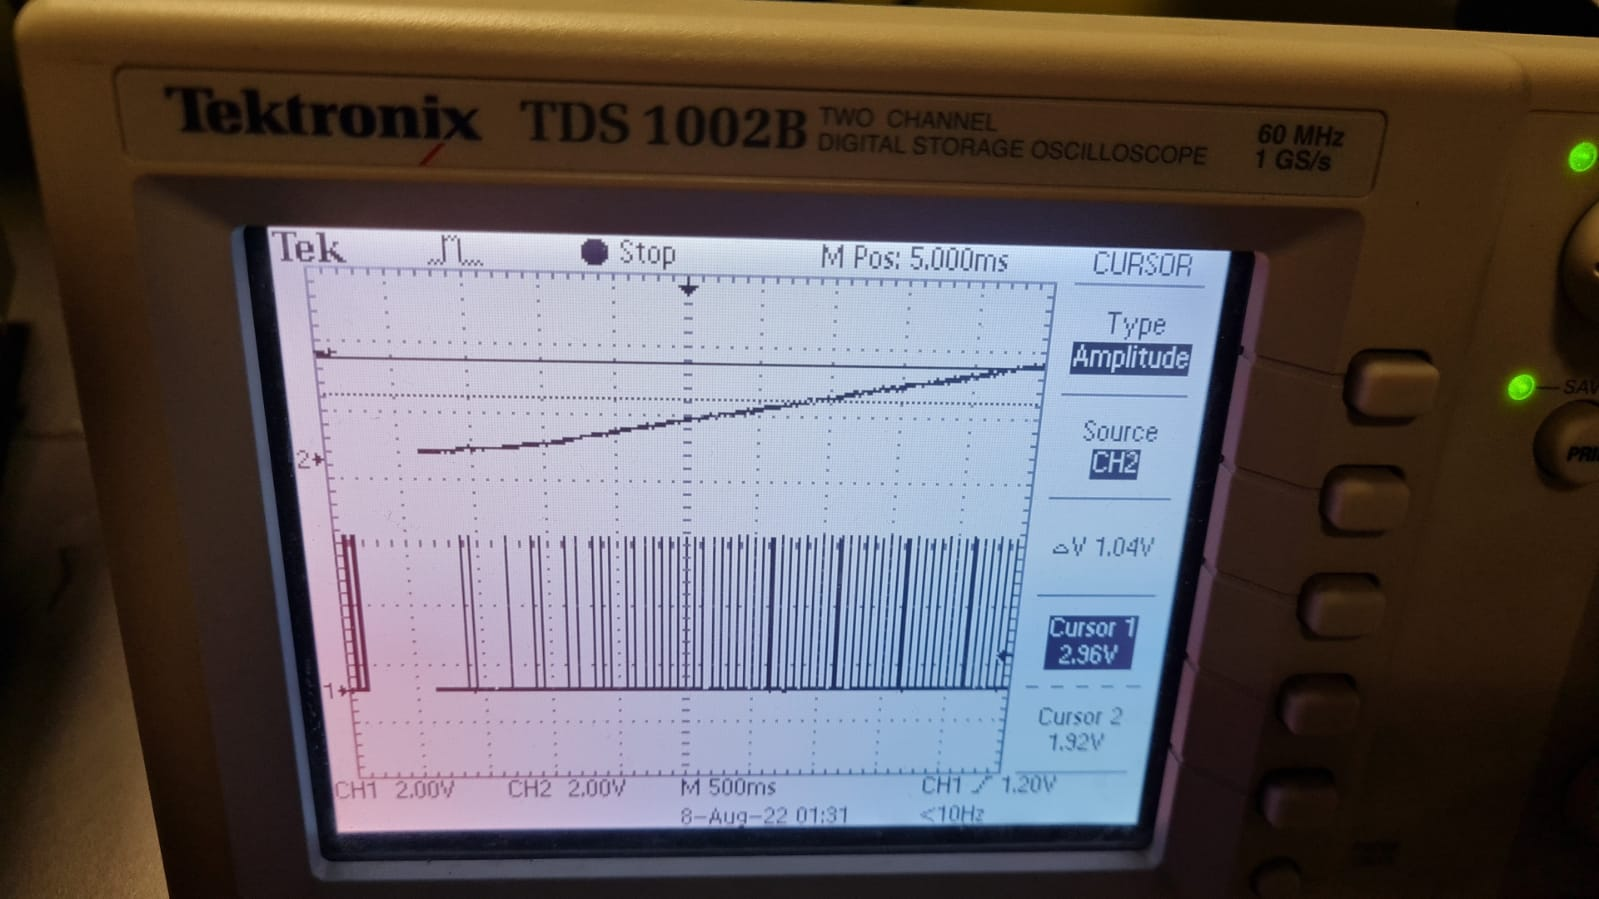
\includegraphics[width=0.95\textwidth]{rangeSensor_impl_gradual}
        \caption{Gradual Change over Input Range}
        \label{fig:rangeSensor_impl_gradual}
    \end{minipage}
\end{figure}

Similarly, the implementation of the circuit also complied with specifications:
\begin{itemize}
    \item Figure \ref{fig:rangeSensor_impl_noiseLevel} indicates a noise level of $\SI{64}{mV_{pp}}$. Although this is only measured at
          \SI{1.76}{V} output, it seems the oscilloscope was struggling to provide accurate readings and could not be zoomed in further.
    \item Figure \ref{fig:rangeSensor_impl_stepResponse} indicates a rise time of around 300 ms.
    \item Figure \ref{fig:rangeSensor_impl_gradual} shows the gradual response of the circuit. The cursor is on 2.96 V in the Figure, and
          by counting divisions it can be seen that it began at around 0.2 V. This shows a relatively linear response.
\end{itemize}